\documentclass[../../main.tex]{subfiles}
\begin{document}

\begin{flushright}
\footnotesize\textit{【自動文字起こし・要確認】}
\end{flushright}

[解] まず、半径$r$について $0 < r < \dfrac{1}{2}$ が必要である。 $\cdots$ ①

\begin{center}
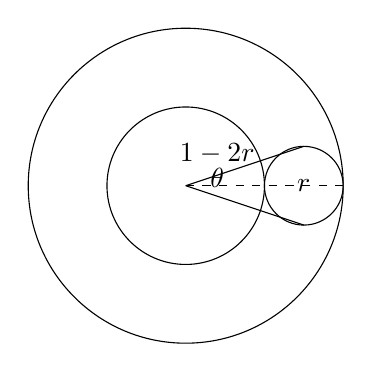
\begin{tikzpicture}[scale=2]
\draw (0,0) circle (1);
\draw (0,0) circle (0.5);
\node at (0.2, 0.2) {$1-2r$};
\draw (0.75, 0) circle (0.25);
\node at (0.75, 0) {$r$};
\draw[dashed] (0,0) -- (1,0);
\draw (0,0) -- (0.75, 0.25);
\draw (0,0) -- (0.75, -0.25);
\node at (0.2, 0.05) {$\theta$};
\end{tikzpicture}
\end{center}

(1) 上図のように半径$r$の円を順に$C_1, C_2, \cdots$とし、その中心を$O_1, O_2, \cdots$とする。又、図のように$\theta$をおくと
$$ \sin \theta = \dfrac{r}{1-r} \quad \cdots \text{②} $$
である。又、円が$n$コあることから$\theta$について
\begin{align}
2n\theta &\le 2\pi \\
\therefore \quad \theta &\le \dfrac{\pi}{n} \quad \cdots \text{③}
\end{align}
$n \ge 2$から $\dfrac{\pi}{n} \le \dfrac{\pi}{2}$ であり $0 \le \theta \le \pi/2$ で $\sin \theta$ が単調増加することから、②③より
$$ \dfrac{r}{1-r} \le \sin \dfrac{\pi}{n} $$
$r$についてといて、①とあわせて
$$ 0 < r \le \dfrac{\sin \dfrac{\pi}{n}}{1+\sin \dfrac{\pi}{n}} $$

(2) $n+2$コの円の面積の総和$S_n(r)$とおくと
\begin{align}
\dfrac{S_n(r)}{\pi} &= 1 + (1-2r)^2 + nr^2 \equiv f_n(r) \\
f_n'(r) &= 2nr + 8r - 4 \\
&= 2 \{(n+4)r - 2\} \quad \cdots \text{④}
\end{align}
である。

[補題]
$$ g(x) = \dfrac{\sin x}{1+\sin x}, \quad h(x) = \dfrac{2x}{\pi+4x} \text{について} \left(0 < x \le \dfrac{\pi}{2}\right) $$
$$ g(x) > h(x) $$
$g(x) = 1 - \dfrac{1}{1+\sin x}, \quad h(x) = \dfrac{1}{2} - \dfrac{\pi}{2(\pi+4x)}$ より
$F(x) = g(x) - h(x)$ とおくと
$$ F'(x) = - \dfrac{\cos x}{(1+\sin x)^2} + \dfrac{\pi}{2} \dfrac{-4}{(4x+\pi)^2} \le 0 \quad \left(\because 0 < x \le \dfrac{\pi}{2}\right) $$
より $F(x)$ は単調減少。これと $F(\pi/2) = \dfrac{1}{2} > 0$ から $F(x) > 0$ なので補題は示された。

[補題] から下表をえる
\begin{center}
\begin{tabular}{|c|c|c|c|c|c|}
\hline
$r$ & $0$ & $\cdots$ & $\dfrac{2}{n+4}$ & $\cdots$ & $\dfrac{\sin \dfrac{\pi}{n}}{1+\sin \dfrac{\pi}{n}}$ \\
\hline
$S'$ & & $-$ & $0$ & $+$ & \\
\hline
$S$ & & $\searrow$ & & $\nearrow$ & \\
\hline
\end{tabular}
\end{center}
よってもとめる$r$は $r = \dfrac{2}{n+4}$ である。

\end{document}
